\section{Teste de localização com smartphone}
\label{sec:teste-smarphone}

Para verificar a capacidade do sensores de localizar contextualmente um
dispositivo móvel, smartphone, foi utilizado. Este foi posicionado em duas salas
diferentes, em cada uma das salas foi executada uma captura de 10 minutos. Para
que houvesse tráfego na rede o dispositivo móvel foi configurado para receber um
stream de vídeo no aplicativo \emph{Netflix}.

\begin{figure}[htb]
	\caption{\label{fig-planta-baixa}Ambiente de teste}
	\begin{center}
		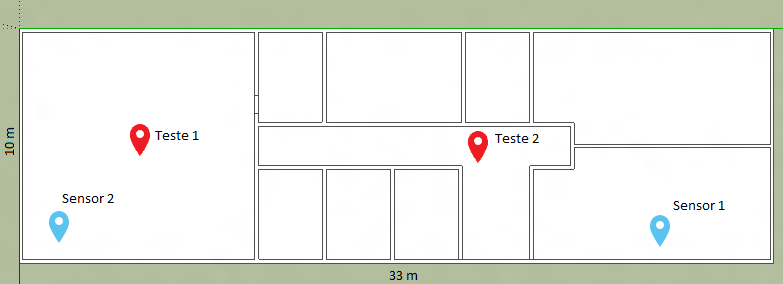
\includegraphics[width=1\textwidth]{060-testes/data-analisis/planta-baixa-smartphone.png}
	\end{center}
	\legend{Fonte: Elaborada pelo autor}
	\nota[Em azul]{Sensores da aplicação}%
	\nota[Em vermelho]{Pontos do dispositivo teste}%
\end{figure}


No teste 1 o dispositivo estava na mesma sala do sensor 2, as distâncias
aproximadas em metros entre o ponto de teste e o sensor 1 é de \texttt{21,52m} e
entre o memso ponto e o sensor 2 é de \texttt{7,00m}. Foram capturados
\texttt{157 736} pacotes totalizando \texttt{9,7 MB} pelo sensor 1 e \texttt{21
974} pacotes totalizando \texttt{1.9 MB} de captura pelo sensor 2.

Para o teste 2 o dispositivo móvel estava posicionado no corredor fora da sala
do sensor 1 e distante do sensor 2, as distâncias aproximadas em metros entre o
ponto de teste e o sensor 1 é de \texttt{9,35m} e entre o memso ponto e o sensor
2 é de \texttt{20,14m}. Neste teste o sensor 1 capturou \texttt{103 555} pacotes
totalizando \texttt{6.4 MB}  de captura e o sensor 2 capturou \texttt{22 635}
pacotes totalizando \texttt{2 MB} de captura.

Posteriormente os arquivos de captura foram analisados com a ferramenta
\emph{Ron’s Editor} para que um sumário fosse construído.

\clearpage
\begin{figure}[ht]
	\centering
	\caption{\label{fig-mg4-noise-t1}Sumário de pacotes por dispositivo - Teste 1}
	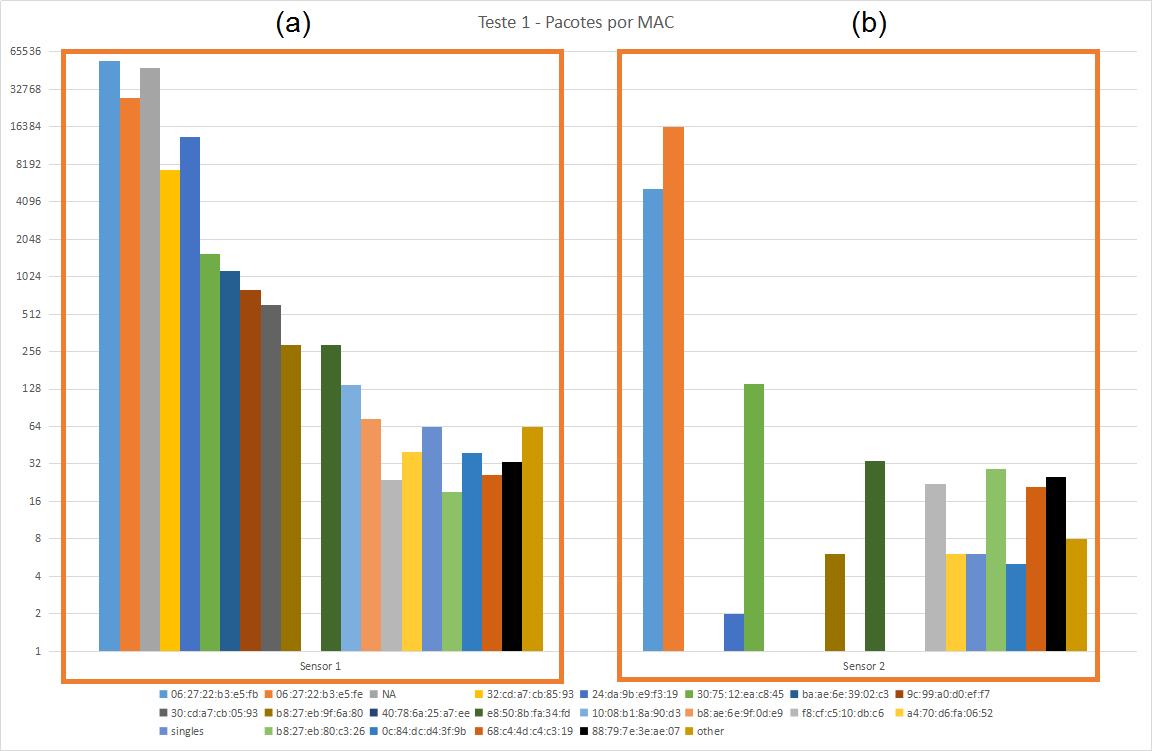
\includegraphics[height=0.32\textheight,width=1\textwidth]{060-testes/data-analisis/distance-mg4plus-netflix/Teste1.png}
	\legend{A esquerda os pacotes recebidos pelo sensor 1 e a direita do sensor 2.
	Em preto o dispositivo de teste.
	Fonte: Elaborada pelo autor}
\end{figure}

\begin{figure}[hb]
	\centering
	\caption{\label{fig-mg4-noise-t2}Sumário de pacotes por dispositivo - Teste 2}
	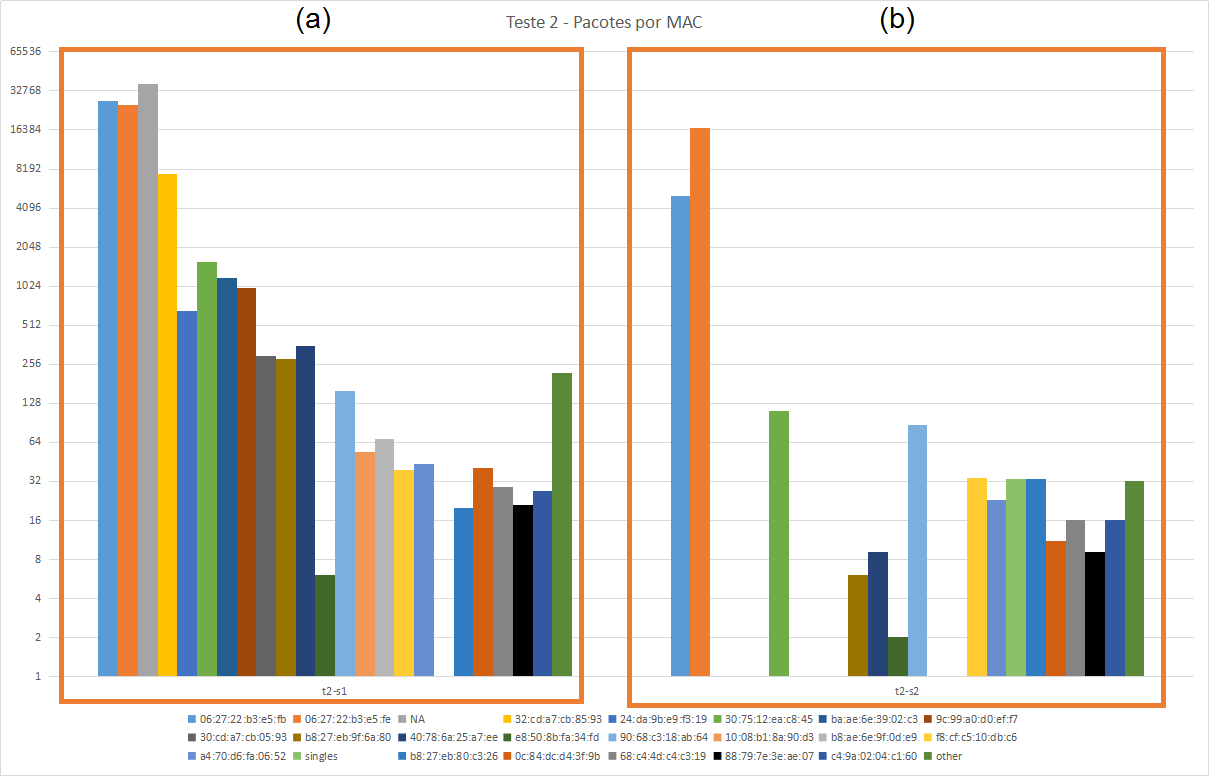
\includegraphics[height=0.32\textheight,width=1\textwidth]{060-testes/data-analisis/distance-mg4plus-netflix/Teste2.png}
	\legend{A esquerda os pacotes recebidos pelo sensor 1 e a direita do sensor 2.
	Em preto o dispositivo de teste.
	Fonte: Elaborada pelo autor.}
\end{figure}

Pode-se obeservar que o \emph{smartphone} não representa a maioria dos pacotes
capturados, evidenciando a constatação do ambiente real e ruidozo em que o teste foi
executado.

\clearpage

Porém, uma vez filtrado os pacotes onde o endereço MAC do transmissor é o do
\emph{smartphone} podemos inferir os valores médios e o desvio padrão, chegando
nos seguinte valores.

\begin{table}[htb]
\IBGEtab{%
\ABNTEXchapterfont {
	\caption{\label{table:smartphone-distance}Análise dos pacotes do \emph{smartphone} - 10 minutos}%
}
}{%
\begin{tabular}{c|cc|cc}
\toprule
\midrule
Teste							& \multicolumn{2}{c|}{teste 1}			&	\multicolumn{2}{c}{teste 2}	\\
\midrule
Sensor 							&	Sensor 1		&	Sensor 2		&	Sensor 1		&	Sensor 2	\\
\midrule
Pacotes							&	33				&	25				&	21				&	9			\\
$\overline{dBm}$				&	-76.6969697		&	-49.88			&	-53.95238095	&	-68.55555556\\
$\sigma$						&	2.833778931		&	2.833137248		&	4.177034719		&	3.431876714	\\
\midrule
\midrule
$d(\overline{dBm})$				&	68.36730882		&	3.118889584		&	4.984470702		&	26.77797784	\\
$d(\overline{dBm} - \sigma)$	&	49.33550049		&	2.250832294		&	3.081536468		&	18.03781557	\\
$d(\overline{dBm} + \sigma)$	&	94.74088372		&	4.321722353		&	8.062519603		&	39.75315605	\\
Erro acumulado metros			&	45.40538323		&	2.070890059		&	4.980983136		&	21.71534048	\\
\midrule
\midrule
Distância real $M$				&	21.52			&	7				&	9.35			&	20.14		\\
$d(\overline{dBm}) - M$			&	46.84730882		&	3.881110416		&	4.365529298		&	6.637977837	\\
\midrule
\bottomrule
\end{tabular}%
}{%
	\fonte{Produzido pelo autor.}%
}
\end{table}

Os mesmos padrões encontrados na \autoref{sec:teste-ruido} aparecem: desvio
padrão grande, erro acumulado maior ainda.

Porém este trabalho limita-se a determinar o contexto (sala) esta resposta pode
ser vista no contraste das \autoref{fig-mg4-t1} e \autoref{fig-mg4-t2} onde a
mudança do contexto é mais clara.

\begin{figure}[htb]
	\label{mg4-distance}
	\centering
	\begin{minipage}{0.49\textwidth}
	\centering
		\caption{\label{fig-mg4-t1}dBm Motorola G4+ - Teste 1}
		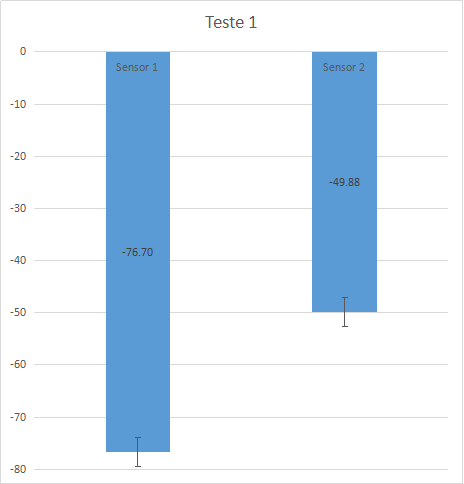
\includegraphics[width=1\textwidth]{060-testes/data-analisis/distance-mg4plus-netflix/target-Teste1.png}
		\legend{Fonte: Elaborada pelo autor}
	\end{minipage}
	\hfill
	\begin{minipage}{0.49\textwidth}
	\centering
		\caption{\label{fig-mg4-t2}dBm Motorola G4+ - Teste 2}
		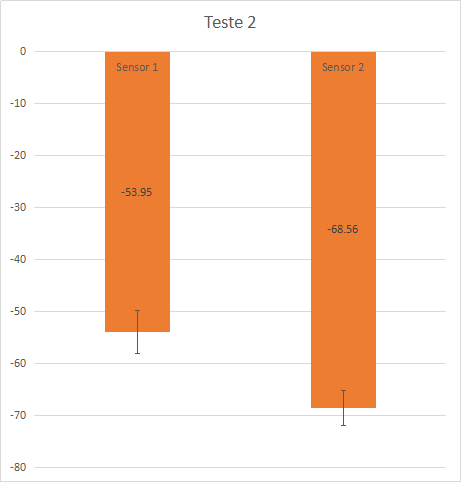
\includegraphics[width=1\textwidth]{060-testes/data-analisis/distance-mg4plus-netflix/target-Teste2.png}
		\legend{Fonte: Elaborada pelo autor}
	\end{minipage}
\end{figure}
